\documentclass[10pt,twocolumn]{article}

\usepackage[utf8]{inputenc}
\usepackage[T1]{fontenc}
\usepackage[margin=0.85in]{geometry}
\usepackage{graphicx}
\usepackage{amsmath}
\usepackage{booktabs}
\usepackage{hyperref}
\usepackage{caption}
\usepackage{titlesec}

\hypersetup{colorlinks=true, linkcolor=blue, urlcolor=blue, citecolor=blue}

\titleformat{\section}{\normalfont\large\bfseries}{\thesection.}{0.5em}{}
\titleformat{\subsection}{\normalfont\bfseries\itshape}{\thesubsection.-}{0.4em}{}

\setlength{\parindent}{0pt}
\setlength{\parskip}{0.5em}

\begin{document}

\twocolumn[
  \begin{center}
    {\LARGE\bfseries Sleep vs GPA in College: Predecir el Promedio Académico del Semestre}\\
    \vspace{0.8em}
    {\large Emilio López}\\
    {\small A01711977@tec.mx}
    \vspace{1.2em}
  \end{center}

  \noindent\textbf{ABSTRACT} Este reporte muestra cómo construimos, a mano y con gradiente descendiente, un modelo de regresión lineal múltiple para predecir el GPA del semestre (\textit{term\_gpa}) de estudiantes universitarios a partir de datos de sueño y variables demográficas, usando el dataset \textit{``Sleep vs GPA in College''}. Durante la limpieza de datos encontramos y corregimos duplicados, una fuga de información y varias columnas redundantes, y comparamos dos formas de tratar los datos nulos en las variables de carga académica, uno fue imputarlos con la mediana y el otro fue simplemente quitar esas filas. El modelo final, llegó a un R$^2$ de 0.462 en training y 0.424 en test con la estrategia de imputación, superando en ambos casos a la estrategia de eliminar las filas (R$^2$ de 0.412 y 0.392). Esto sugiere que el modelo capta una parte de la variabilidad del GPA, sobre todo gracias al GPA previo del estudiante, y que todavía hay espacio para mejorar con modelos no lineales, que es justo lo que se propone como siguiente paso.
  \vspace{1.5em}
]

\section{Introducción}

El sueño es uno de los factores que más se ha estudiado en relación con el rendimiento académico. Dormir poco o tener horarios de sueño muy irregulares se ha relacionado consistentemente con menos capacidad de concentración, memoria y desempeño académico en estudiantes universitarios. Pero el desempeño de un estudiante no depende solo de cómo duerme, cosas como su historial académico, cuántos créditos está cursando y su contexto demográfico también importan.

El objetivo de este trabajo es armar, desde cero y sin usar librerías de modelado como \texttt{scikit-learn}, un modelo de regresión lineal múltiple que prediga el GPA del semestre (\textit{term\_gpa}) de un estudiante a partir de sus patrones de sueño, su historial académico y variables demográficas. La idea no es solo llegar a un modelo que funcione, sino mostrar todo el proceso de limpieza, transformación y modelado de datos, incluyendo decisiones importantes como detectar fugas de información y comparar distintas formas de tratar los datos nulos.

\section{Descripción del Dataset}

El dataset principal, \textit{college\_sleep\_and\_gpa.csv}, es de Kaggle~\cite{kaggle_dataset} y tiene 634 filas, cada una es el registro de un estudiante en un semestre en específico. También hay un dataset de referencia, \textit{study\_cohort\_reference.csv}, que describe las cohortes (\textit{study}, \textit{university}, \textit{semester}, \textit{cohort\_code}) y cuántos estudiantes tiene cada una.

\subsection{Features}

El dataset tiene 22 columnas, entre las que destacan:

\begin{itemize}
  \setlength\itemsep{0.1em}
  \item \textbf{student\_id}: identificador del estudiante (no único entre universidades).
  \item \textbf{cohort\_code}: código de la cohorte (universidad + semestre + estudio).
  \item \textbf{gender, first\_generation, underrepresented}: variables demográficas.
  \item \textbf{avg\_sleep\_hours, daytime\_sleep\_minutes, sleep\_midpoint\_minutes, bedtime\_variability, nights\_tracked\_fraction}: variables de sueño.
  \item \textbf{prior\_gpa}: GPA acumulado antes del semestre.
  \item \textbf{term\_gpa}: GPA del semestre (\textbf{variable objetivo}).
  \item \textbf{gpa\_change}: diferencia entre \textit{term\_gpa} y \textit{prior\_gpa}.
  \item \textbf{term\_units, term\_load\_z}: carga académica del semestre (créditos y carga normalizada).
\end{itemize}

\section{Extracción y Limpieza de Datos}

\subsection{Duplicados}

Al revisar duplicados por \textit{student\_id} encontramos varias coincidencias. Pero al investigar esas filas vimos que en realidad eran estudiantes de \textbf{distintas universidades} que por casualidad compartían el mismo número de id, no registros duplicados de verdad. Para confirmarlo armamos una llave compuesta, \textit{student\_uid} (\textit{cohort\_code} + \textit{student\_id}), y con esa sí dio cero duplicados, cada fila era efectivamente un estudiante distinto.

\subsection{Valores Nulos}

Las columnas \textit{gender}, \textit{first\_generation} y \textit{underrepresented} tenían muy pocos nulos (menos del 1\%), así que simplemente quitamos esas filas sin que afectara casi nada el tamaño del dataset.

\textit{term\_units} y \textit{term\_load\_z}, en cambio, tenían bastantes más nulos. Como no estaba claro qué estrategia era mejor, decidimos hacer \textbf{dos versiones del dataset} y comparar cuál funcionaba mejor en el modelo final:

\begin{itemize}
  \setlength\itemsep{0.1em}
  \item \textbf{df\_imputado} (626 filas): los nulos de \textit{term\_units}/\textit{term\_load\_z} se rellenaron con la mediana de cada columna.
  \item \textbf{df\_eliminado} (481 filas): se quitaron las filas que tenían nulos en esas columnas.
\end{itemize}

\subsection{Columnas Redundantes y Fuga de Información}

Encontramos y quitamos 9 columnas por ser redundantes, estar derivadas de otras, o directamente filtrar información de la variable objetivo:

\begin{itemize}
  \setlength\itemsep{0.1em}
  \item \textbf{gpa\_change}: es literalmente \textit{term\_gpa} $-$ \textit{prior\_gpa}, o sea que es una fuga directa de la variable objetivo. Quitarla no era solo por cuestión de limpieza, era necesario para que el modelo no hiciera trampa.
  \item \textbf{study, university, semester}: con tablas de contingencia vimos que tienen un mapeo 1:1 con \textit{cohort\_code}, así que no aportaban nada nuevo.
  \item \textbf{avg\_sleep\_minutes, sleep\_midpoint\_clock, under\_6h\_sleep, sleep\_bracket}: son la misma información en otro formato (cambio de unidad, de formato, o agrupada en rangos) de columnas que ya teníamos (\textit{avg\_sleep\_hours} y \textit{sleep\_midpoint\_minutes}).
  \item \textbf{student\_id}: ya lo reemplazamos con \textit{student\_uid}, y como identificador puro no aporta nada al modelo.
\end{itemize}

\section{Transformación de Datos}

\subsection{Análisis de Correlación}

Calculamos la matriz de correlación de Pearson sobre las variables numéricas de \textit{df\_imputado} (Figura~\ref{fig:corr}). La variable más correlacionada con \textit{term\_gpa} fue, por mucho, \textit{prior\_gpa} ($r = 0.638$), seguida de \textit{sleep\_midpoint\_minutes} ($r = -0.197$), \textit{underrepresented} ($r = -0.173$) y \textit{avg\_sleep\_hours} ($r = 0.206$). Esto deja claro que el historial académico previo es el mejor predictor lineal que tenemos, mientras que las variables de sueño, al contrario de lo que pensabamos, aportan algo pero mucho más débil.

\begin{figure}[h]
  \centering
  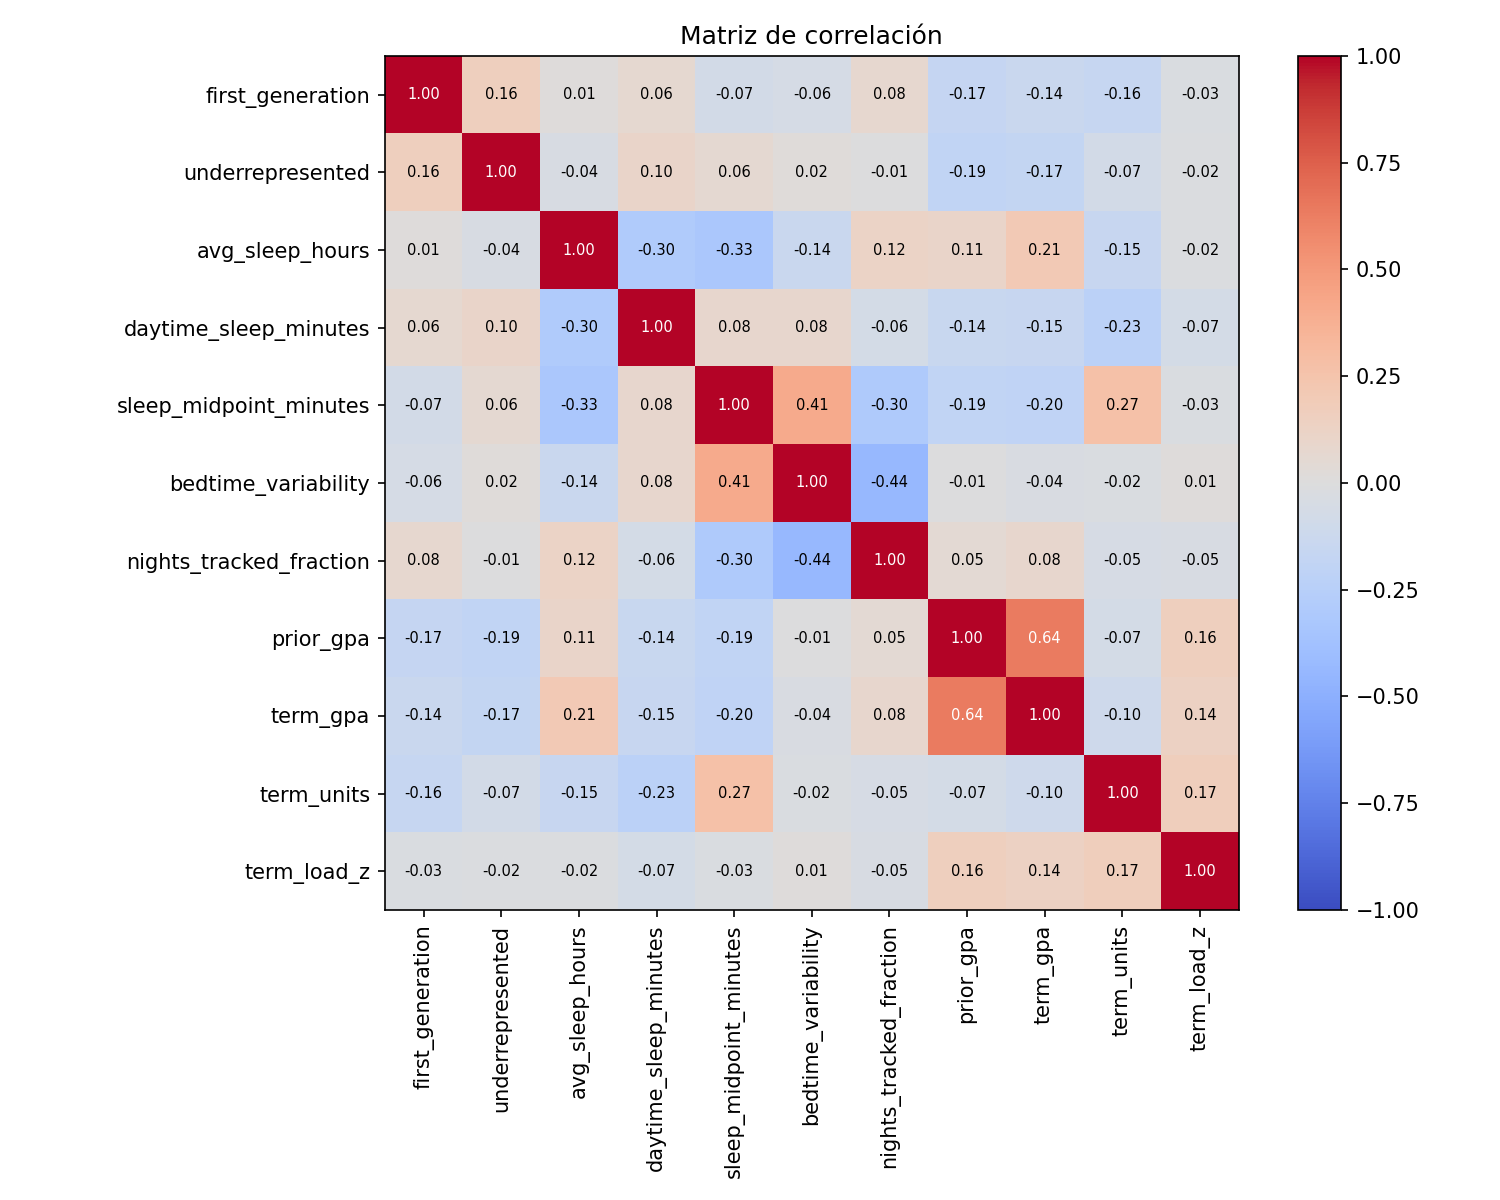
\includegraphics[width=\linewidth]{correlation_heatmap.png}
  \caption{Matriz de correlación entre las variables numéricas del dataset.}
  \label{fig:corr}
\end{figure}

La Figura~\ref{fig:disp} muestra cada predictor numérico contra \textit{term\_gpa} por separado, y confirma a simple vista que \textit{prior\_gpa} es la única variable con una tendencia lineal clara.

\begin{figure*}[t]
  \centering
  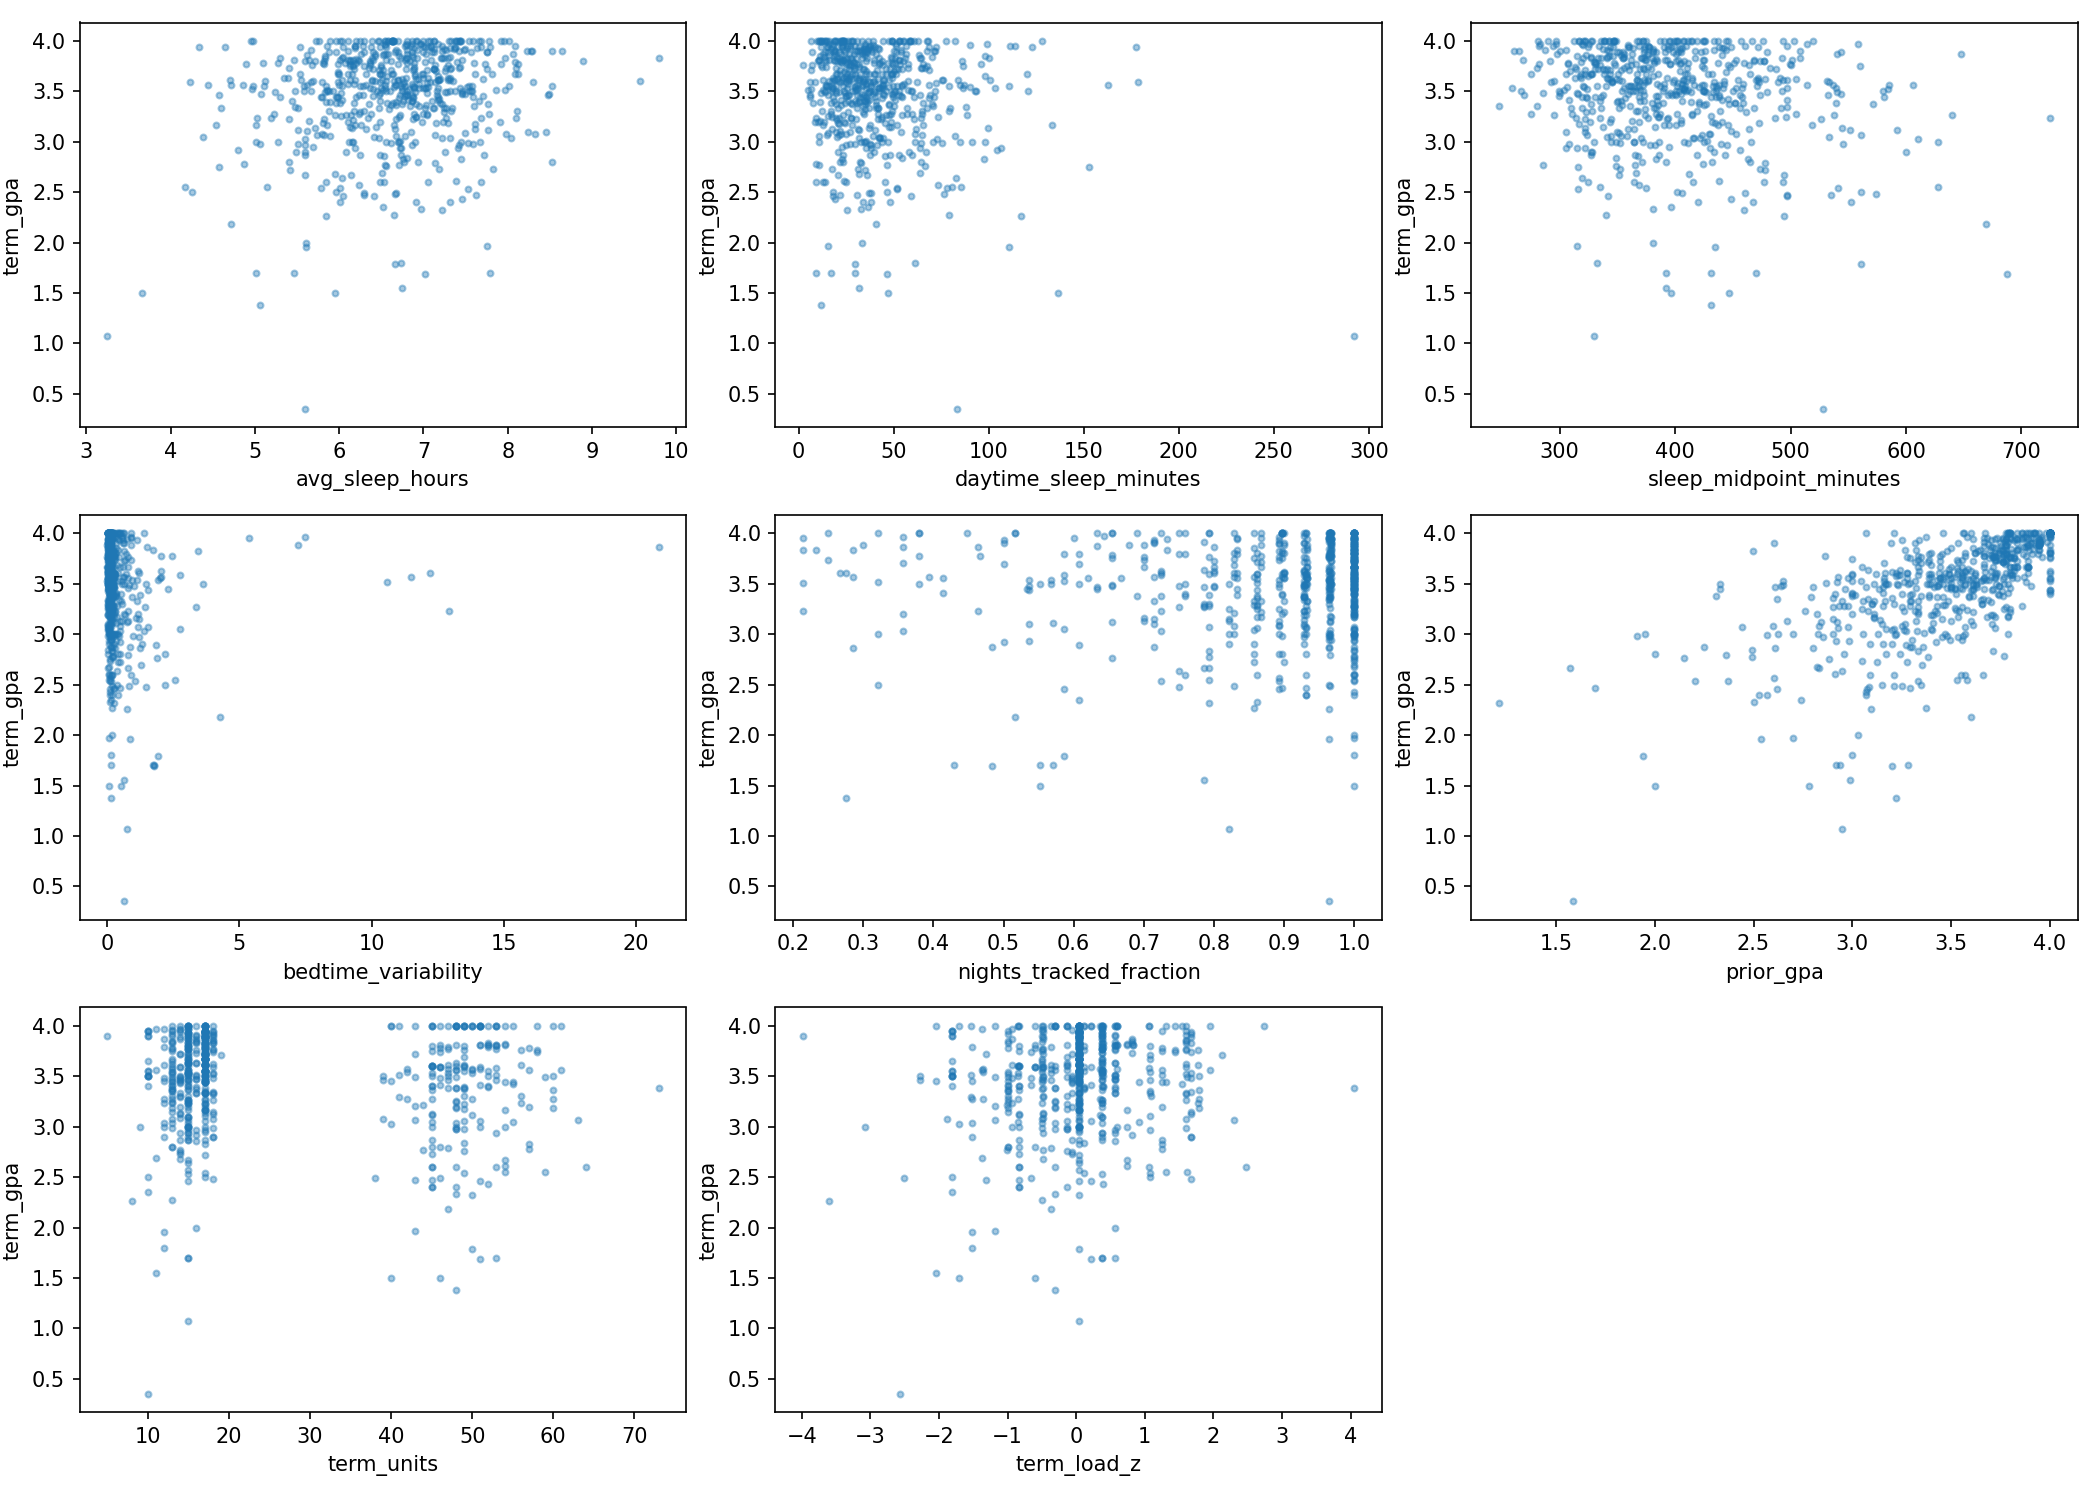
\includegraphics[width=0.85\textwidth]{dispersion.png}
  \caption{Dispersión de cada variable numérica contra \textit{term\_gpa}.}
  \label{fig:disp}
\end{figure*}

También comparamos \textit{term\_gpa} entre cohortes (Figura~\ref{fig:cohorte}) y sí hay diferencias reales: las medias van de 3.28 a 3.66 según la universidad, así que vale la pena conservar \textit{cohort\_code} como predictor. En cambio, la diferencia de \textit{term\_gpa} por género fue casi nula (3.449 contra 3.452), así que esa variable probablemente no aporte mucho.

\begin{figure}[h]
  \centering
  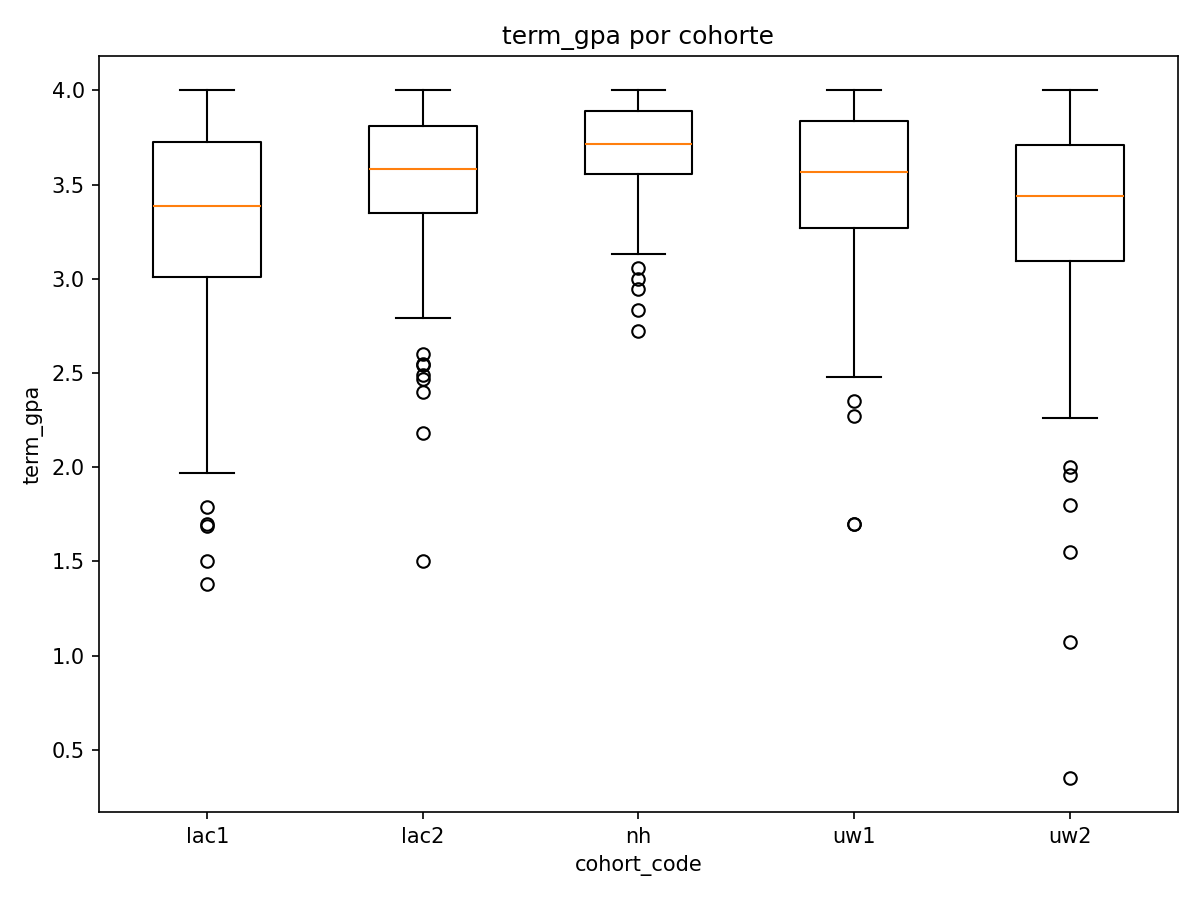
\includegraphics[width=\linewidth]{gpa_por_cohorte.png}
  \caption{Distribución de \textit{term\_gpa} por cohorte.}
  \label{fig:cohorte}
\end{figure}

\subsection{Codificación de Variables Categóricas}

Las variables categóricas de texto (\textit{gender} y \textit{cohort\_code}) se convirtieron a columnas binarias de 0 y 1 con \textit{One-Hot Encoding}, usando \texttt{drop\_first=True} para que las columnas dummy no queden perfectamente correlacionadas entre sí (si no, la regresión tendría columnas linealmente dependientes).

\subsection{Escalamiento}

Antes de entrenar, estandarizamos todas las variables predictoras a media 0 y desviación 1. Importante: la media y desviación usadas para escalar el conjunto de prueba se calcularon \textbf{solo con el conjunto de training}, para no filtrar información del test hacia el entrenamiento.

\subsection{División del Dataset}

Dividimos el dataset al azar en 80\% para entrenamiento y 20\% para prueba, con una semilla fija para que sea reproducible. Esto se hizo por separado tanto para \textit{df\_imputado} como para \textit{df\_eliminado}.

\section{Construcción y Evaluación del Modelo}

\subsection{Selección de Features y Variable Objetivo}

Usamos todas las columnas que quedaron después de la limpieza (menos \textit{term\_gpa}) como predictoras, y \textit{term\_gpa} como variable objetivo. Entrenamos y evaluamos el modelo por separado en \textit{df\_imputado} y \textit{df\_eliminado}, para ver cómo afecta la estrategia de tratar nulos al resultado final.

\subsection{Hipótesis}

La hipótesis del modelo es simplemente una combinación lineal de las predictoras más un término de sesgo (\textit{bias}):
\begin{equation}
h(x) = x \cdot \theta + b
\end{equation}
donde $\theta$ es el vector de coeficientes y $b$ es el sesgo, que manejamos como un parámetro aparte en vez de agregar una columna de puros unos.

\subsection{Función de Costo}

Usamos el Error Cuadrático Medio (MSE) como función de pérdida:
\begin{equation}
J(\theta, b) = \frac{1}{m}\sum_{i=1}^{m}\left(h(x_i) - y_i\right)^2
\end{equation}

\subsection{Descenso de Gradiente}

Los parámetros arrancan en cero y se van actualizando, iteración tras iteración, en dirección contraria al gradiente de la función de costo:
\begin{align}
\theta &:= \theta - \alpha \cdot \frac{1}{m} X^T (h(X) - y) \\
b &:= b - \alpha \cdot \frac{1}{m} \sum_{i=1}^{m} (h(x_i) - y_i)
\end{align}
con una tasa de aprendizaje $\alpha = 0.01$. El entrenamiento para cuando el $R^2$ de entrenamiento llega a 0.95 o cuando se cumplen 10,000 épocas (al momento de ejecutarlos, ambos modelos corrieron las 10,000 épocas completas sin poder llegar al umbral de 0.95).

\subsection{Evaluación del Modelo}

El desempeño se evaluó con $R^2$ y RMSE:
\begin{equation}
R^2 = 1 - \frac{\sum(y - \hat{y})^2}{\sum(y - \bar{y})^2}, \quad \text{RMSE} = \sqrt{\frac{\sum(y-\hat{y})^2}{m}}
\end{equation}

\section{Visualización y Resultados}

La Tabla~\ref{tab:resultados} nos muestra el desempeño final de ambas estrategias de tratamiento de datos nulos.

\begin{table}[h]
\centering
\small
\begin{tabular}{lcccc}
\toprule
\textbf{Dataset} & \textbf{Train R$^2$} & \textbf{Test R$^2$} & \textbf{Train RMSE} & \textbf{Test RMSE} \\
\midrule
df\_imputado  & 0.462 & \textbf{0.424} & 0.370 & \textbf{0.373} \\
df\_eliminado & 0.412 & 0.392 & 0.396 & 0.469 \\
\bottomrule
\end{tabular}
\caption{Comparación de desempeño entre las estrategias de imputación con la mediana y eliminación de las filas.}
\label{tab:resultados}
\end{table}

\textit{df\_imputado} le ganó a \textit{df\_eliminado} en las dos métricas. Lo más notable es que su diferencia entre error de train y test (0.370 a 0.373) es casi nula, mientras que \textit{df\_eliminado} tiene una diferencia más grande (0.396 a 0.469), esto probablemente porque su conjunto de entrenamiento es más chico (481 filas contra 626). Con esta evidencia, \textbf{la imputación con la mediana es la estrategia recomendada} por encima de eliminar las filas.

\begin{figure*}[t]
  \centering
  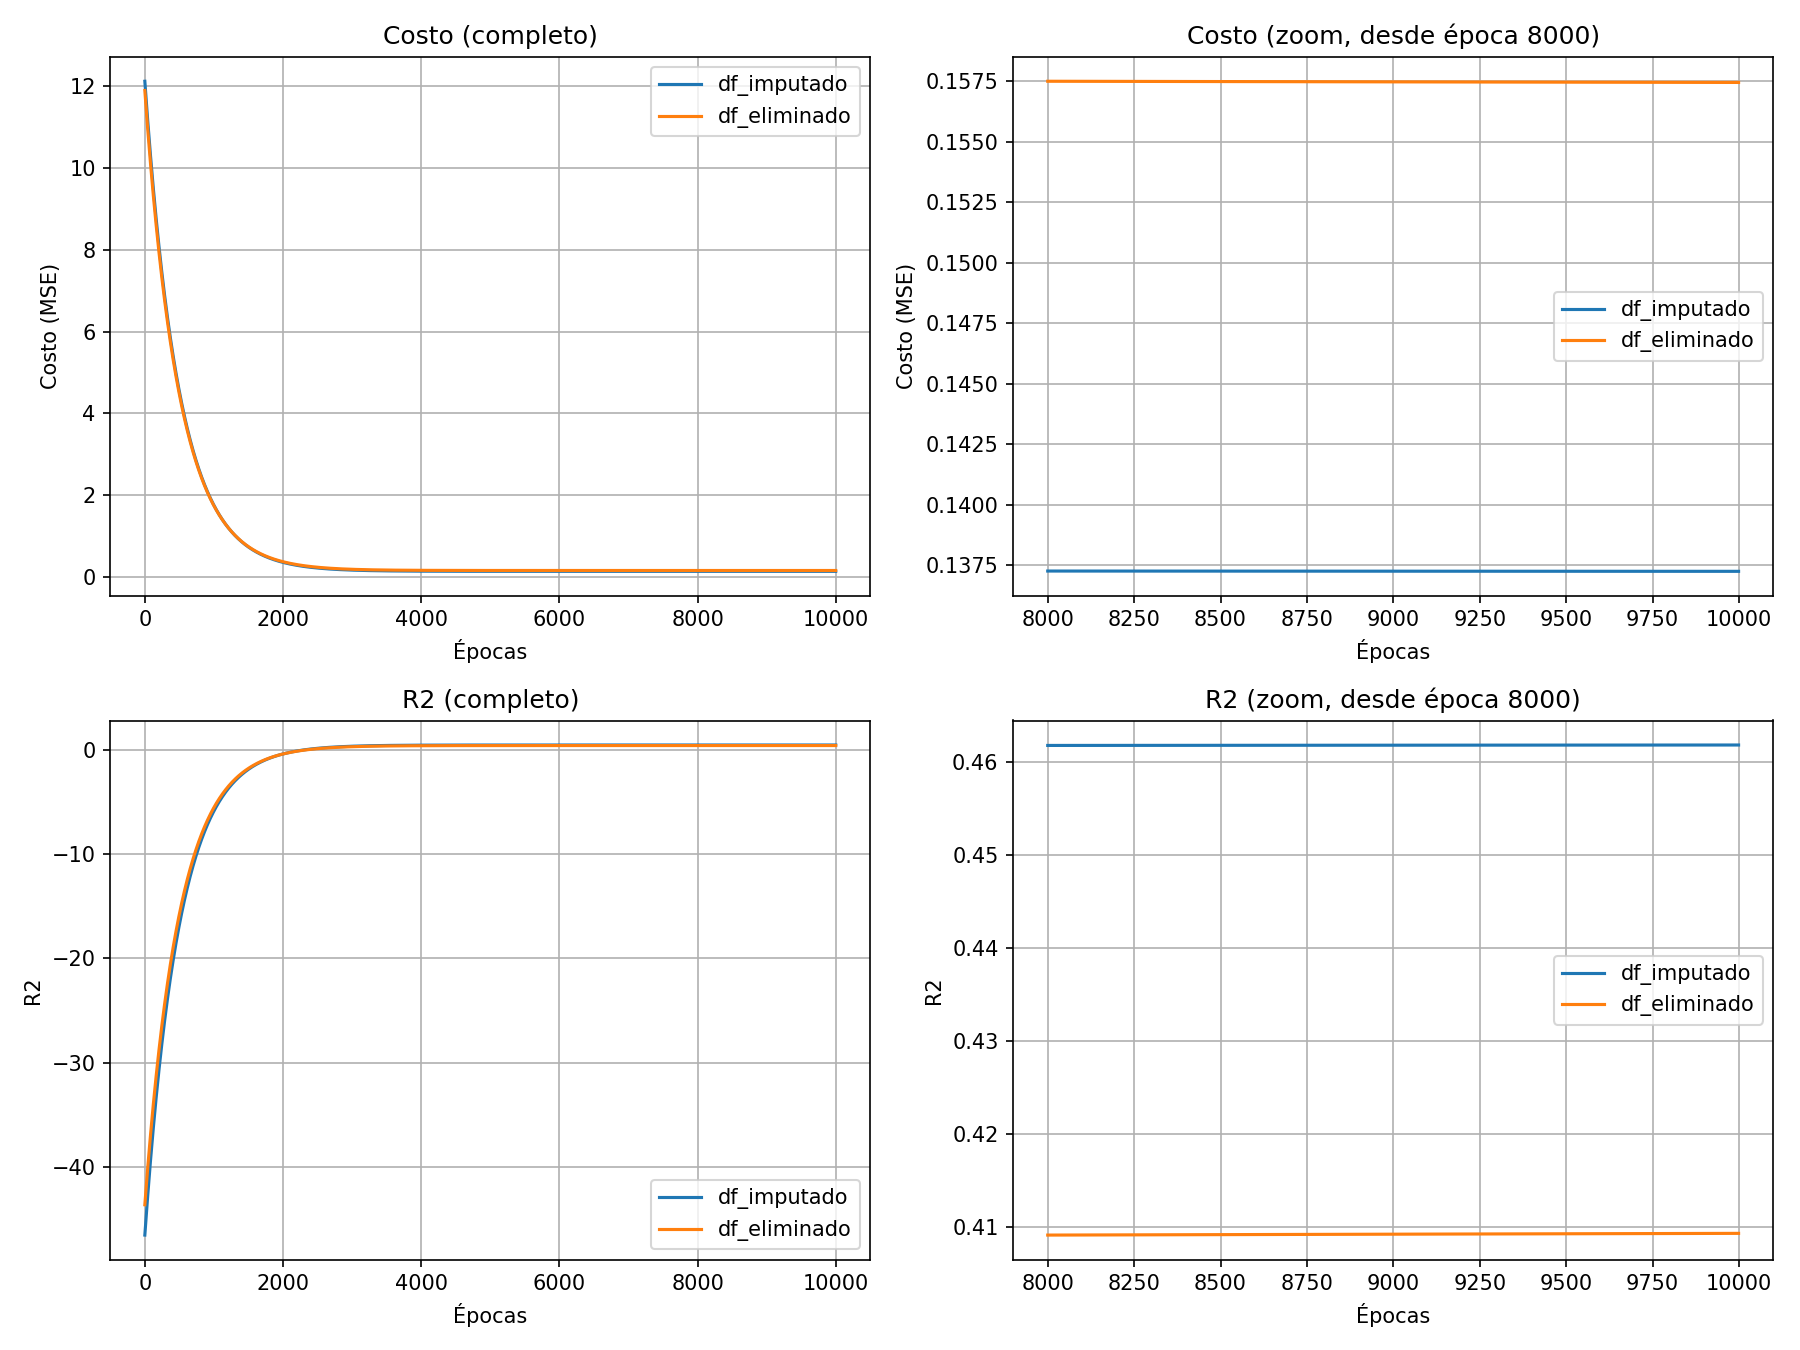
\includegraphics[width=0.85\textwidth]{curvas_entrenamiento.png}
  \caption{Curvas de costo y $R^2$ durante el entrenamiento, completas y con zoom en el último 20\% de las épocas, para ambas estrategias de imputación.}
  \label{fig:curvas}
\end{figure*}

La Figura~\ref{fig:curvas} muestra que los dos modelos convergen bastante rápido (antes de la época 500), y que la ventaja de \textit{df\_imputado} se mantiene estable durante todo el entrenamiento.

\begin{figure*}[t]
  \centering
  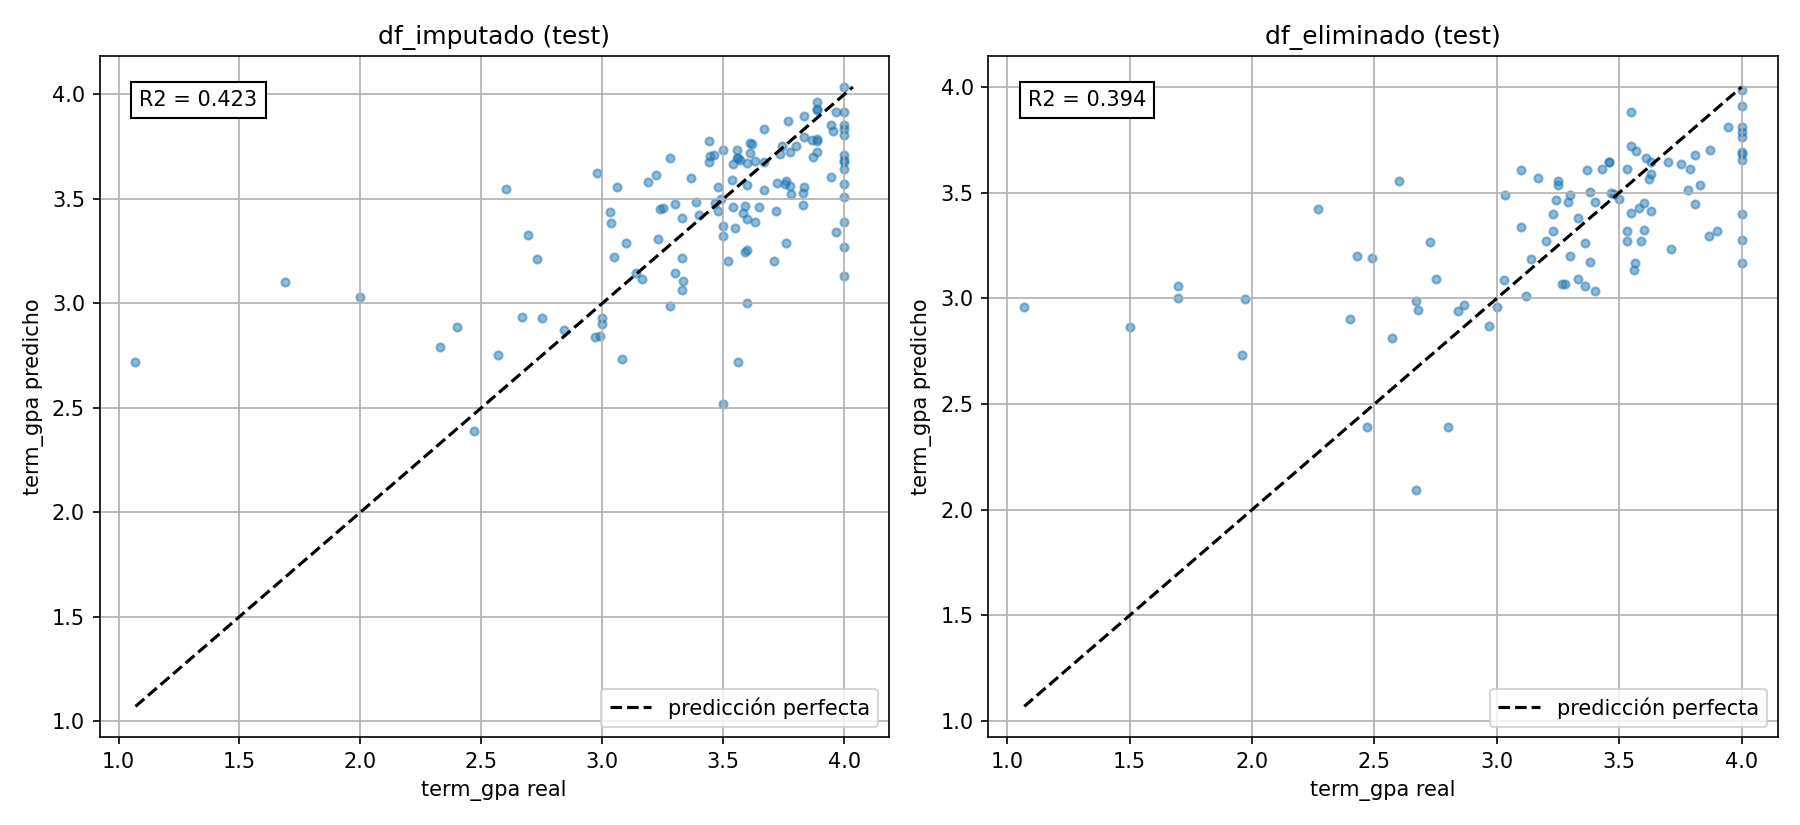
\includegraphics[width=0.85\textwidth]{prediccion_vs_real.png}
  \caption{Predicción del modelo contra el valor real de \textit{term\_gpa} sobre el conjunto de prueba, para ambas estrategias.}
  \label{fig:pred}
\end{figure*}

La Figura~\ref{fig:pred} muestra el comportamiento típico de un modelo con $R^2$ moderado: para GPAs bajos (1.0--2.5) el modelo sobreestima casi siempre, y para GPAs altos (cerca de 4.0) hay bastante dispersión. Esto tiene sentido con un modelo que capta la tendencia general pero le cuesta con los extremos, un indicio de \textbf{underfitting} moderado.

\section{Siguientes Pasos: Implementación con Framework}

Como siguiente paso, la idea es reimplementar este mismo problema con un framework de \textit{Machine Learning} (por ejemplo, \texttt{scikit-learn}) para:

\begin{itemize}
  \setlength\itemsep{0.2em}
  \item \textbf{Validar la implementación manual}: entrenar un \texttt{LinearRegression} (solución cerrada) con los mismos datos y checar que dé coeficientes y $R^2$/RMSE parecidos a los que sacamos a mano con descenso de gradiente.
  \item \textbf{Explorar modelos no lineales}: como el $R^2$ actual ($\approx$0.42) sugiere que una relación puramente lineal no está capturando toda la señal, probar modelos como \texttt{RandomForestRegressor} o \texttt{GradientBoostingRegressor}, que podrían agarrar interacciones no lineales entre sueño, carga académica y GPA previo.
  \item \textbf{Comparar bias y varianza} entre el modelo lineal a mano y los del framework, con el mismo esquema train/test, para saber si el problema es \textit{underfitting} o si el techo de $R^2$ viene de que los datos de sueño son ruidosos por naturaleza.
\end{itemize}

Con esa comparación vamos a saber si vale la pena aumentar la complejidad del modelo, o si el modelo lineal que ya tenemos está cerca del límite de lo que se puede explicar con estas variables.

\renewcommand{\refname}{Referencias}
\begin{thebibliography}{1}
\small
\bibitem{kaggle_dataset} Feng, K. (n.d.). \textit{Sleep vs GPA in College}. Kaggle. \url{https://www.kaggle.com/datasets/kylefengkfeng209/sleep-vs-gpa-in-college/data}
\end{thebibliography}

\end{document}
